\newpage
\chapter*{Úvod} % normalni kapitola \chapter{kapitola}
\addcontentsline{toc}{chapter}{Úvod}

%\textit{Ekaterina Eremenko}

Za úkol na předmětu Projektové Praktikum bylo zadáno navrhnout a následně sestrojit aparaturu pro urychlování svazku elektronů, což zahrnuje návrh a realizaci zapojení elektronového děla, zdroje vysokého napětí, doplňující soustavu fokusující svazek a v neposlední řadě samotný detektor intenzity elektronového svazku \cite{PanMysak, Kralik}.   

\begin{figure}[htbp!]
\centering
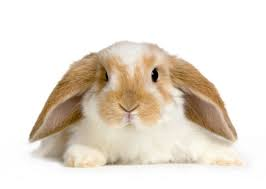
\includegraphics[width = 170 pt]{Figure/kralik.jpeg}
\hfill

\includegraphics[scale = 0.5]{Figure/mysak.jpeg}
 \caption{Kralík a Pan Myšák před začátkem projektu.}
\label{02ukazka}
\end{figure}


